\documentclass[10pt]{article}
\usepackage[margin=0.8in]{geometry}
\usepackage{graphicx}
\usepackage{xcolor}
\usepackage{enumitem}
\usepackage{microtype}
\usepackage{titlesec}
\usepackage{parskip}
\usepackage{float}

% ── Color Palette ──
\definecolor{userblue}{HTML}{1A237E}
\definecolor{layerlabel}{HTML}{37474F}
\definecolor{accentgray}{HTML}{546E7A}

% ── Section styling ──
\titleformat{\section}{\large\bfseries\color{userblue}}{\thesection}{1em}{}
\titleformat{\subsection}{\normalsize\bfseries\color{accentgray}}{\thesubsection}{1em}{}

\begin{document}

\title{\textbf{SBI SecureTrust: A Multi-Layered Defense Architecture\\Against Counterfeit Banking Applications}}
\date{}
\maketitle

\begin{center}
\textit{\small Keywords:\ Mobile Banking Security $\cdot$ Fake App Detection $\cdot$ FIDO2 Passkeys $\cdot$ Anti-Phishing $\cdot$ Behavioral Security $\cdot$ Fraud Prevention}
\end{center}

\vspace{0.4cm}

\section*{Abstract}

\noindent
Counterfeit mobile banking applications---distributed via SMS, WhatsApp, and third-party APK channels---represent a rapidly growing fraud vector in India. By mimicking legitimate bank interfaces, these apps enable credential theft, unauthorized access, and large-scale financial loss. Existing defenses such as OTP-based authentication and app store vetting remain fundamentally reactive and insufficient against modern social engineering and sideloading attacks.

We present \textbf{SBI SecureTrust}, a proactive, multi-layered architecture that intervenes at every stage of the fraud lifecycle. The system comprises six complementary defense layers:

\begin{enumerate}[leftmargin=*, itemsep=1pt, parsep=0pt, topsep=4pt]
    \item \textbf{Cryptographically Signed QR Distribution:} Replaces link-based app discovery with tamper-proof sources anchored to the bank's signing keys.
    \item \textbf{Behavioral Friction Engine:} Disrupts social engineering via anti-coaching challenges, enforced reboots, and time-delayed sideloading gates.
    \item \textbf{On-Device Fake App Detection:} Uses perceptual similarity analysis and origin attestation to neutralize impersonating apps before execution.
    \item \textbf{FIDO2 Passkey Authentication:} Eliminates phishing and credential replay with hardware-bound, origin-scoped cryptographic passkeys.
    \item \textbf{Vernacular Behavioral Nudges:} Delivers real-time, risk-calibrated voice warnings in the user's native language.
    \item \textbf{AI-Driven Brand Monitoring:} Continuously scans app stores and phishing infrastructure to trigger automated takedowns.
\end{enumerate}

\noindent
A \textbf{real-time fraud containment engine} complements these layers through graph-based intelligence for instant fund freezing, mule account detection, and cross-institutional alert propagation.

\vspace{0.15cm}
\noindent
\textbf{Key Differentiators.}\enspace Unlike conventional single-point solutions, SBI SecureTrust unifies \emph{cryptographic trust}, \emph{behavioral security}, and \emph{ecosystem-wide threat intelligence} into a cohesive defense-in-depth framework. The architecture is bank-agnostic and extensible, enabling adoption across India's digital banking ecosystem.

\vspace{0.1cm}
\noindent
\textbf{Impact.}\enspace By shifting fraud prevention from reactive detection to proactive disruption, SBI SecureTrust can substantially reduce losses from counterfeit banking apps, protect vulnerable users, and reinforce trust in mobile-first banking across emerging markets.

\vspace{1.0cm}

% ═══════════════════════════════════════════
% ARCHITECTURE DIAGRAM (Image)
% ═══════════════════════════════════════════
\begin{center}
{\Large\bfseries\color{userblue} System Architecture --- SBI SecureTrust}
\end{center}

\vspace{0.4cm}

\begin{figure}[H]
\centering
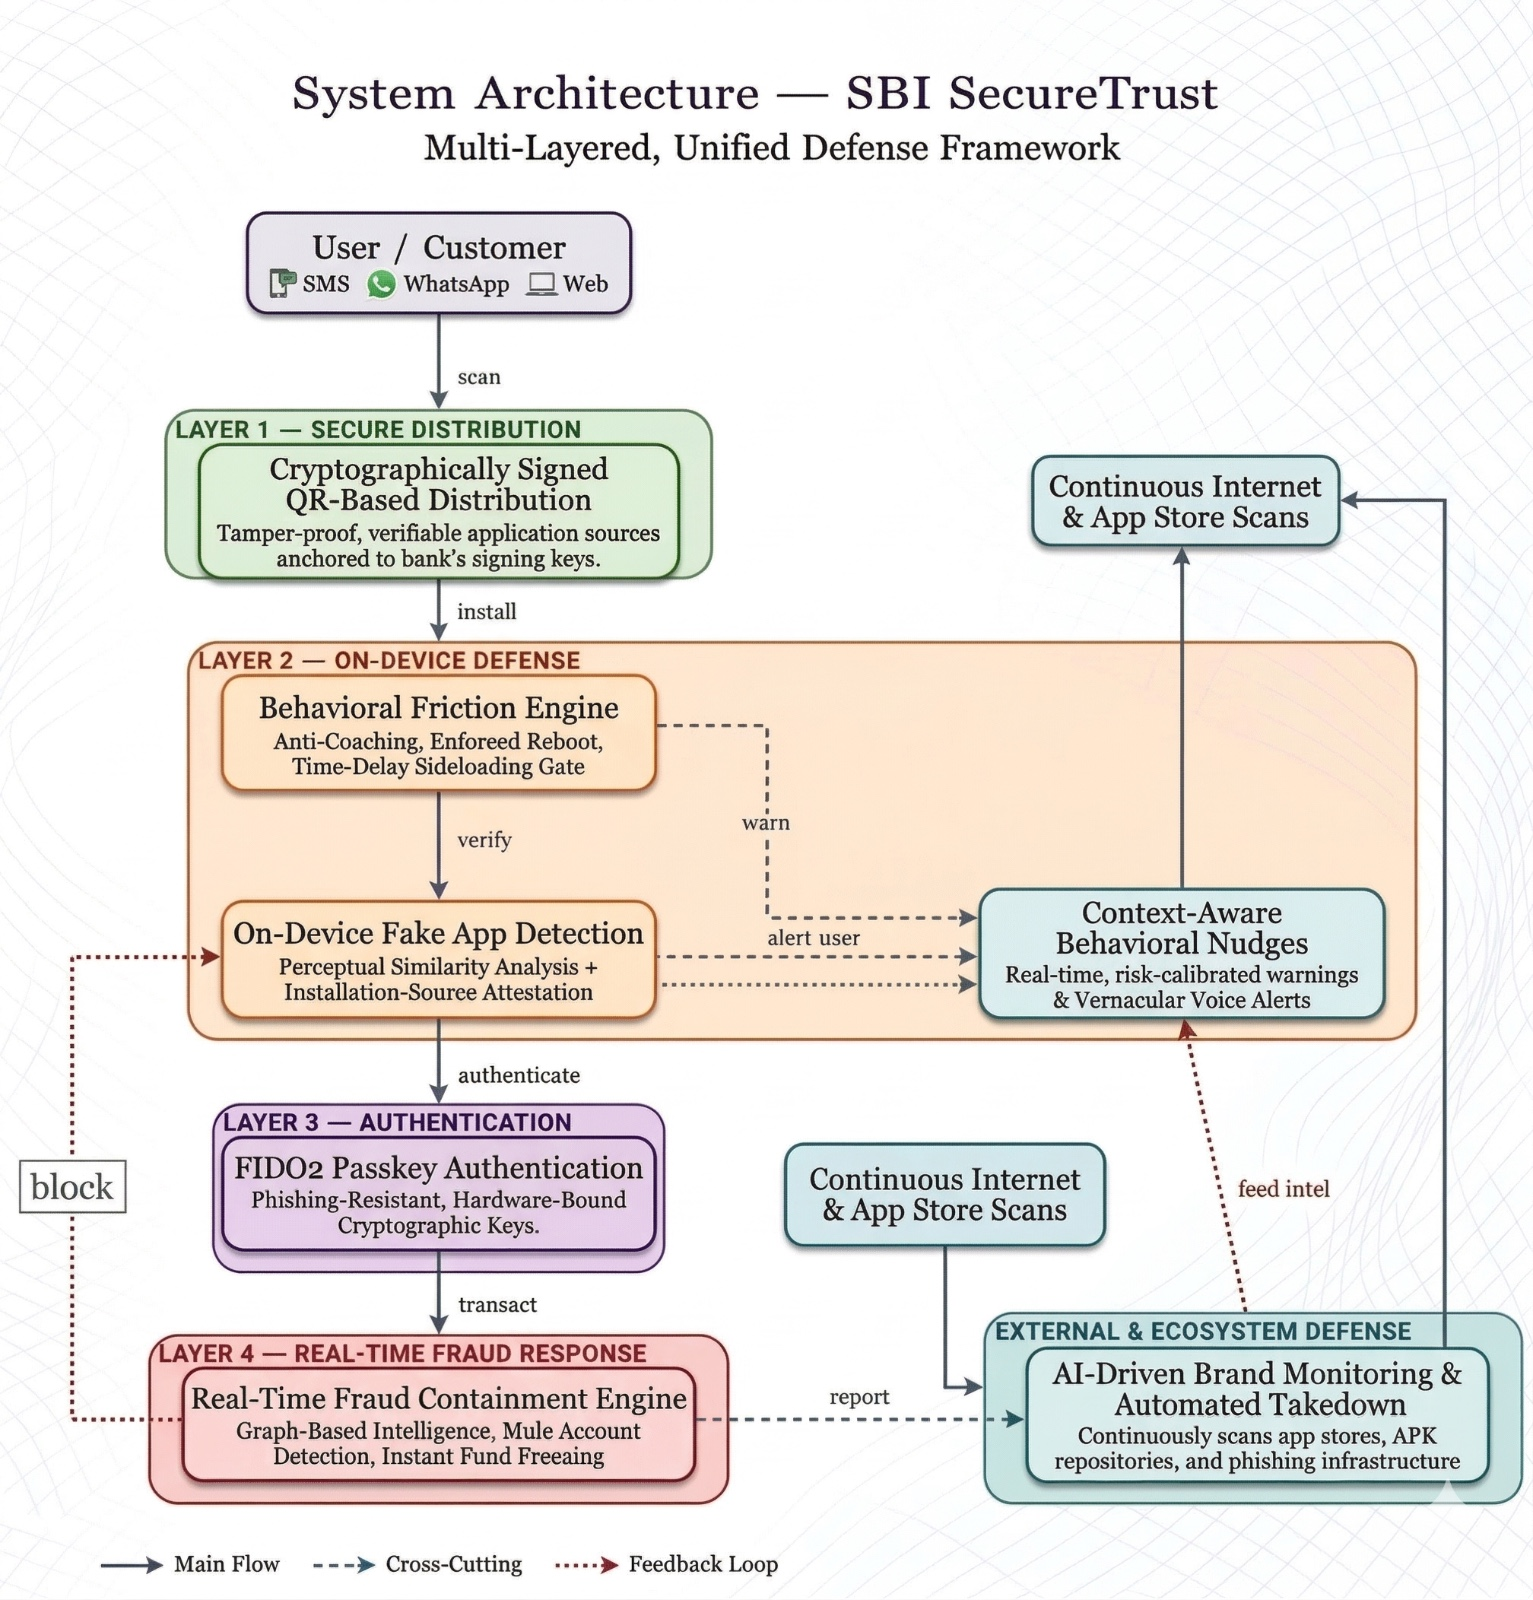
\includegraphics[width=\textwidth]{sbi.jpeg}
\end{figure}

\end{document}
